% Section: Results and Discussion
\section{Results and Discussion}

\subsection{GPR Optimization and Ground-State Identification}

\begin{figure*}
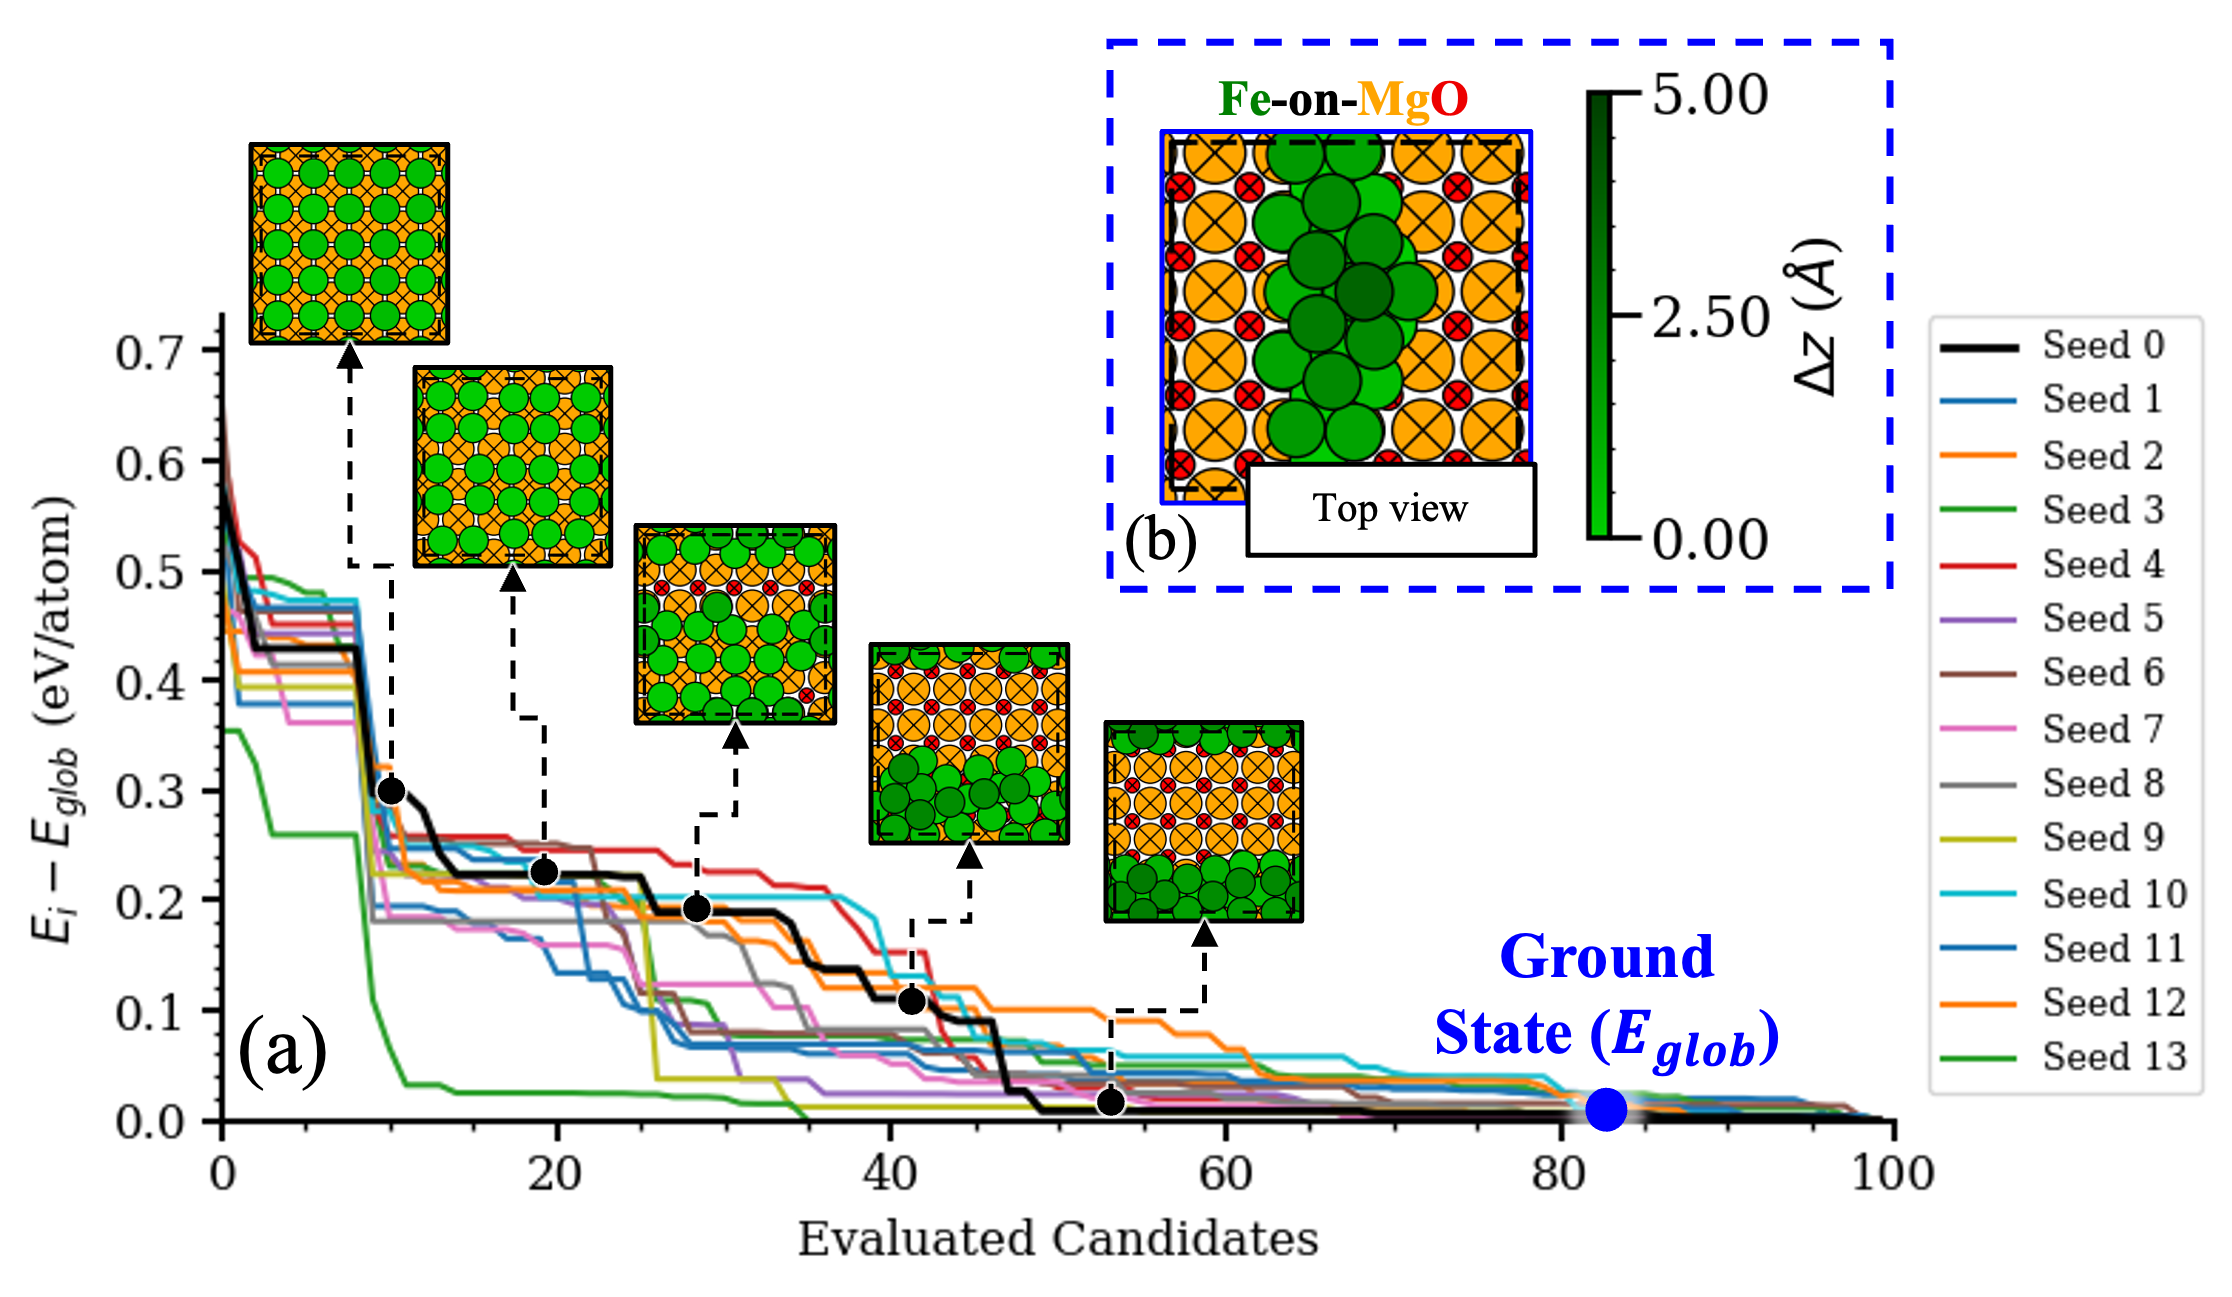
\includegraphics{figures/Fig_Prog.png}
\caption{ \label{fig:eProg} (a) GPR optimization process across 13 independent runs (Run 1–13), tracing the energy difference relative to the ground state ($E_i - E_{\text{glob}}$) against the number of DFT-evaluated candidates. Insets track top-view atomic configurations at key optimization stages along the Run 1 path (black circles), capturing the structural transition from high-energy flat monolayers to lower-energy island phases. (b) Top view of the final island ground state ($E_{\text{glob}}$). The color bar ($\Delta z$) maps the atomic height variation within the Fe layer relative to the substrate, distinguishing flat layers ($0.00\text{ \AA}$) from islands ($\sim 5.00\text{ \AA}$).).
}
\end{figure*}

We first present the GPR optimization results from the sampling process for Fe-on-MgO, as shown in Fig. \ref{fig:eProg}a. The \textit{x}-axis tracks the number of evaluated candidates, which directly corresponds to the progression of the sampling process, indicating the cumulative $M$ evaluated candidates. To ensure structural diversity and assess the robustness of the sampling, the process was further performed using unique randomization seeds (13 independent runs). Because GPR is highly sensitive to the available training data, each sampling process was conducted independently, without sharing databases for the GPR optimization.

The snapshots in Fig. \ref{fig:eProg}a provide top views of the optimization process for Run 1, illustrating the structures of $\text{Fe}$ (green) on the $\text{MgO(001)}$ substrate ($\text{Mg}$ in orange, $\text{O}$ in red). The color gradient on the $\text{Fe}$ atoms represents their relative heights, defined as $\Delta Z = Z_{\text{Fe, top}} - Z_{\text{Fe, bottom}}$, where $Z_{\text{Fe, bottom}}$ corresponds to the $\text{Fe}$ atom closest to the $\text{MgO}$ surface. These snapshots reveal that the high-energy states are predominantly flat-like structures, characterized by a uniform light green color ($\Delta Z \approx 0$). As the energy decreases, the $\text{Fe}$ atoms begin to aggregate, forming the island structures visualized in the later stages of the sampling and highlighted in the ground state ($E_{\mathrm{glob}}$) view. Following the initial 40–50 evaluations, each sampling run reaches an energy plateau near the ground state, typically within $E_i - E_{\text{glob}} \approx 0.0003$ eV/atom. While the specific profile of the energy decline varies between sampling runs, all runs successfully target the same island ground state, confirming that the thermodynamic preference for island is a robust feature of the PES.

For all seeds, each sampling process experiences a sharp drop in energy within the first 10 evaluated candidates—marking the beginning of Phase II—with the energy plateauing and showing no further significant reduction after approximately 80 configurations are evaluated (see Fig. \ref{fig:eProg}a). This rapid minimization observed within Phase II originates from the GPR optimization, which explores the structures based on the dataset established by the small-scale generator in Phase I. Within this framework, we use the small-scale generator exclusively in Phase I to constrain the initial PES exploration to the vicinity of the flat reference configuration rather than starting from completely random arrangements. This choice is intended to establish a physically plausible baseline dataset for the GPR model. Because the GPR surrogate is trained on the Valle-Oganov descriptor, it maps structural fingerprints based on pair potentials, allowing the model to learn these fundamental interactions more efficiently. Then, by incorporating the large-scale generator, the process helps guide the system toward lower-energy structures. Ultimately, starting from Phase II, the introduction of GPR optimization marks the true beginning of local minima sampling across the PES.

We present the ground-state configurations ($E_{\text{glob}}$) for Fe-on-MgO (Fig. \ref{fig:eProg}b), which are intrinsically characterized by the island mode. These findings align with experimental observations where reflection high-energy electron diffraction (RHEED) patterns for thin Fe films exhibit spotty characteristics, indicative of 3D transmission through island-like structures rather than smooth surface scattering \cite{Urano1988}. The tendency toward island formation is further corroborated by scanning tunneling microscopy (STM) studies, which reveal the formation of islands even at elevated growth temperatures \cite{Subagyo2000}. To test the validity of the island ground state, different finite-size supercells were evaluated, alongside testing the reverse deposition of MgO-on-Fe, the details of which are presented in the Supplemental Material.

\begin{figure}
\begin{center}
\begin{tabular}{c}
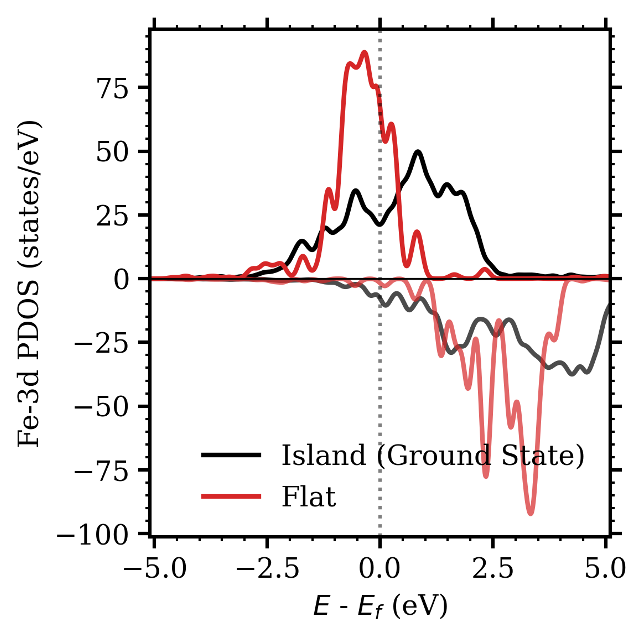
\includegraphics[height=8.5cm]{figures/Fig_dos.png}
\end{tabular}
\end{center}
\caption 
{ \label{Fig_dos} Spin-polarized $\text{Fe}$-$3d$ projected density of states (PDOS) comparing the island ground state (black line) and the flat reference configuration (red line) for $\text{Fe}$ on $\text{MgO(001)}$. Positive and negative values denote the majority (spin-up) and minority (spin-down) channels, respectively. The vertical dotted line at $E - E_f = 0\text{ eV}$ represents the Fermi level.} 
\end{figure} 

The electronic characteristics driving the island mode for Fe-on-MgO were investigated by analyzing the projected density of states (PDOS) for the $\text{Fe } 3d$ orbitals, comparing the ground-state island structure against the reference flat configuration. As shown in Fig. \ref{Fig_dos}, the flat configuration exhibits a sharp peak in the localized $\text{Fe } 3d$ orbitals at the Fermi level ($E - E_f = 0\text{ eV}$), which directly correlates with its elevated total energy. Although these localized orbitals are essential for coherent tunneling in magnetic tunnel junctions (MTJs) \cite{Butler2001}—a mechanism critical for achieving high tunneling magnetoresistance (TMR) \cite{parkin2004, Yuasa2004}—they impose an energy penalty on the uniform thin film.

\subsection{Minimum-Ensemble of Local Minima}

\begin{figure}
\begin{center}
\begin{tabular}{c}
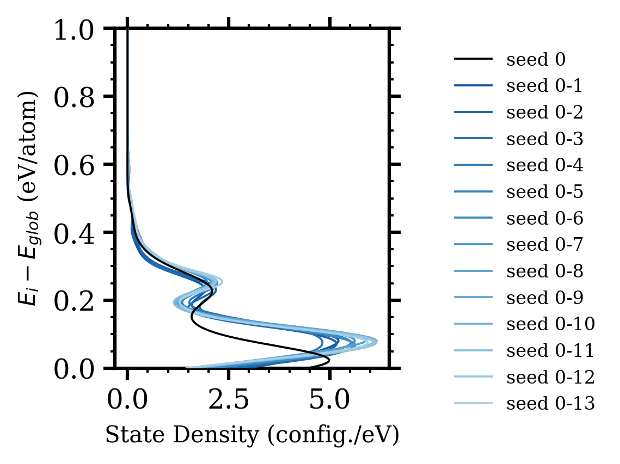
\includegraphics{figures/Fig_convStateDens.png}
\end{tabular}
\end{center}
\caption 
{ \label{Fig_convStateDens} Comparison of the state density distribution $g(E)$ obtained from a single GOFEE search (Run 1, black line) against cumulative distributions formed by sequentially aggregating independent runs (shades of blue).} 
\end{figure} 


To construct a minimum-ensemble of Fe-on-MgO from the evaluated candidates (see Fig. \ref{fig:eProg}a), we aggregate structures generated from Phase II onwards (see Fig. \ref{Fig_flow}). These candidates are GPR optimized and subjected to LCB acquisition to ensure they represent stable local minima on the PES. To estimate the degeneracy profile across different energy levels, we calculate the state density $g(E) = \frac{1}{Mh} \sum_{i=1}^{M} K \left( \frac{E - E_i}{h} \right)$ using Kernel Density Estimation (KDE) \cite{Parzen1962}. Here, $E$ denotes the target energy, $E_i$ the energy of the $i$-th configuration, $K$ the standard Gaussian kernel, and $h$ the smoothing bandwidth defined by Scott's rule, $h = M^{-1/5} \sigma$, where $\sigma$ is the sample standard deviation of the energy dataset.

Due to the stochastic nature of the GPR model, which relies on a random initialization that changes depending on the seed, the sampling process yields slightly different configurations across independent runs. To improve resolution and ensure the accuracy of the calculated $g(E)$, we aggregate the ensembles generated by multiple runs. As shown in Fig. \ref{Fig_convStateDens}, while a single sampling run (Run 1) provides a coarse degeneracy profile distribution, aggregating Runs 1 and 2 shifts the state density peak. However, once the ensembles from Runs 1 to 3 are combined, the overall profile and peak features of $g(E)$ stabilize, remaining largely unchanged with respect to energy upon further data inclusion and verifying statistical convergence.
For maximum statistical resolution, a comprehensive state density was constructed by aggregating all 13 independent sampling runs, resulting in an ensemble of 1,180 DFT-evaluated configurations. The resulting $g(E)$ distribution (Fig. \ref{FigConDis}a) exhibits two distinct peaks of high degeneracy at approximately 0.259 and 0.079 eV/atom. These peaks indicate that the aggregated ensemble captures a diverse PES containing numerous geometrically distinct yet energetically degenerate structures.

\begin{figure*}
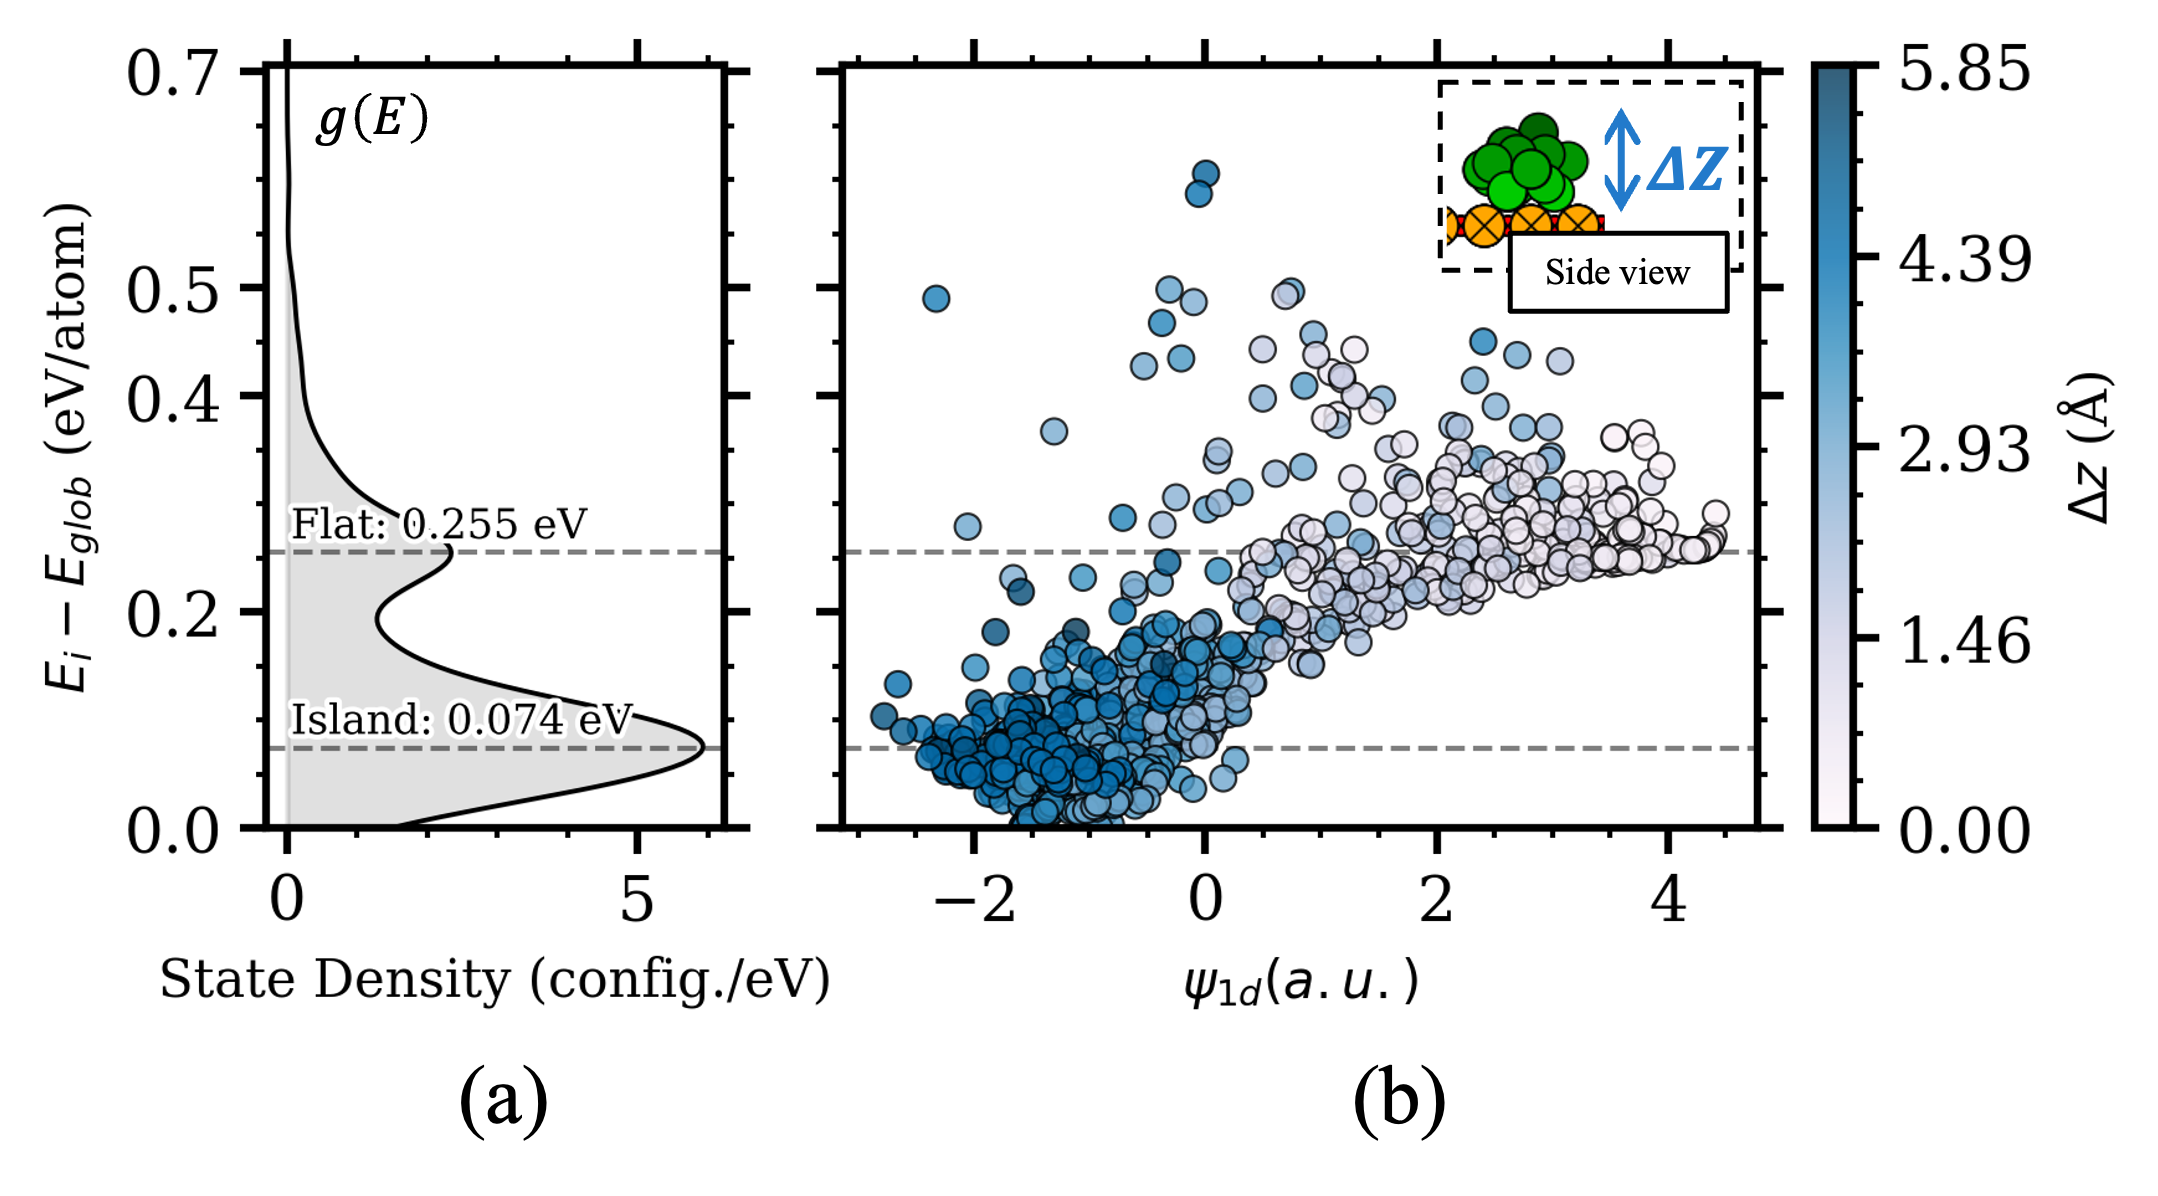
\includegraphics{figures/Fig_ConDen.png}
\caption{ \label{FigConDis} (a) The state density distribution $g(E)$ and (b) the PES mapped using the first principal component ($\psi_{1d}$) from the eigenvalue composition of the Valle-Oganov descriptor \cite{valle2010}. On the left, the distribution identifies two prominent high-degeneracy basins corresponding to the low-energy island phase ($0.079\text{ eV/atom}$) and the high-energy flat phase ($0.259\text{ eV/atom}$). On the right, each point represents a distinct configuration color-coded by the Fe layer height variation $\Delta z$, ranging from flat wetting layers ($0.00\text{ \AA}$, white/light purple) to fully developed 3D clusters ($5.85\text{ \AA}$, dark blue), with horizontal dashed lines visually separating these structural regimes. Note that on the right, the inset illustrates the physical definition of $\Delta z$ via a schematic side view of a deposited island.
}
\end{figure*}

To analyze this ensemble further, we map the PES into a one-dimensional projection, $\psi_{1d}$, as shown in Fig. \ref{FigConDis}b. This dimensionality reduction utilizes an eigendecomposition of the Valle-Oganov descriptor \cite{valle2010}, which constructs a feature matrix $X_{\text{Valle-Oganov}}$ from radial and angular distribution functions. We centered the data to obtain $X_c = X_{\text{Valle-Oganov}} - \bar{X}$ and computed the covariance matrix $C = \frac{1}{M-1} X_c^T X_c$, where $M$ denotes the 1,180 configurations evaluated within the ensemble. The projection is derived by identifying the first eigenvector, $\psi_1$, through the eigenvalue problem $C\psi = \lambda\psi$, representing the principal component that captures the maximum structural variance. By defining $\psi_{1d} = X_c \cdot \psi_1$, the high-dimensional descriptors are projected onto a single axis. Notably, the 0.079 eV/atom region shows a narrow distribution in $\psi_{1d}$ space, suggesting restricted configurational variety at this energy limit, while the 0.259 eV/atom region displays the highest variety, indicating a broader diversity of structural motifs accessible during the transition between growth modes.

To characterize the structural properties of the sampled states, high-degeneracy peaks are mapped to relative island height, $\Delta Z$ (Fig. \ref{FigConDis}b), using the definition from Fig. \ref{fig:eProg}b to distinguish between island and flat phases. The primary peak at 0.079 eV/atom consists of configurations with $\Delta Z$ values between 2.5 Å and 5.0 Å, confirming the thermodynamic stability of the island mode. At the higher energy peak of 0.259 eV/atom, $\Delta Z$ decreases significantly, corresponding to metastable flat configurations. Although these flat structures are energetically less favorable than the island ground state—separated by an energy penalty of approximately 0.18 eV/atom—their manifestation as a distinct degeneracy peak indicates a well-defined local minimum on the PES, rendering them theoretically accessible if the thermodynamic preference is satisfied.

\subsection{Temperature-Dependent Probability}

\begin{figure*}
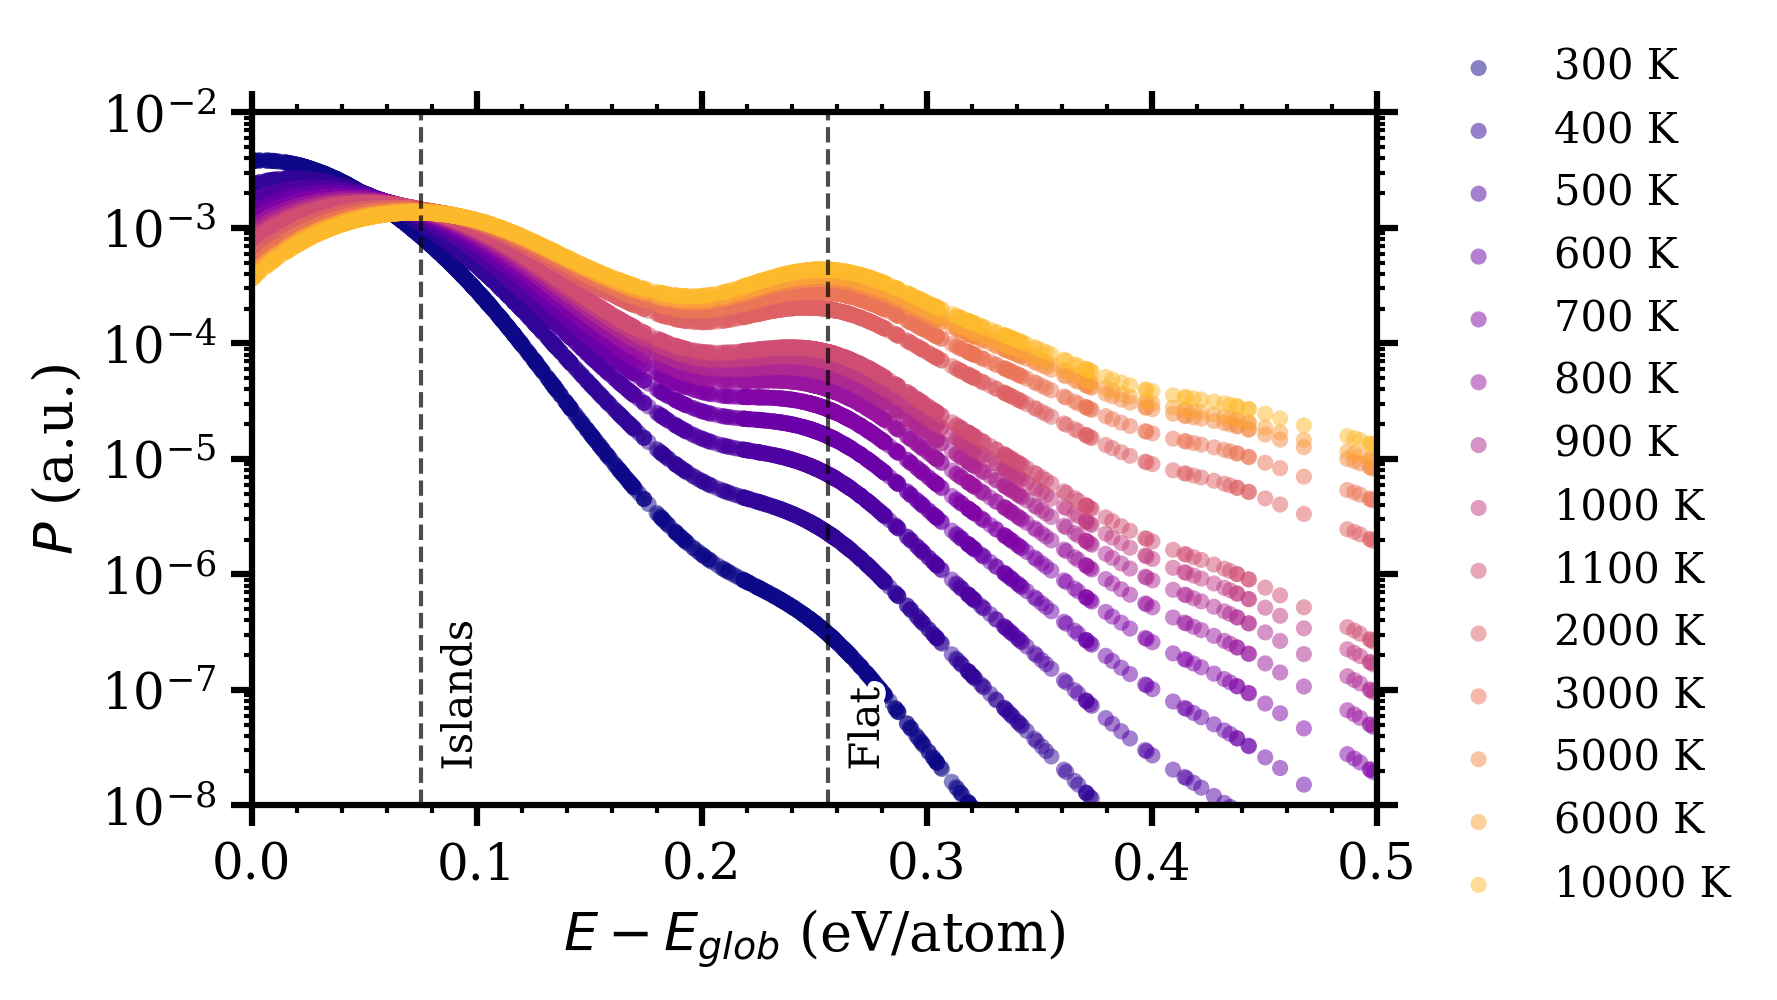
\includegraphics[scale=0.8]{figures/Fig_Boltz.png}
\caption{\label{FigProb} Temperature-dependent Boltzmann probability distribution $P$ as a function of the relative energy per atom $E - E_{glob}$ (eV/atom) for the individual configurations within the minimum-ensemble, weighted against their respective $g(E)$ for the two Fe on MgO(001) phases. The distributions span temperatures from 300 K to 10000 K, indicated by the color gradient from dark blue to light yellow. Vertical dashed lines correspond to high degeneracy points in $g(E)$, identifying the structural configurations labeled as "Islands" at approximately 0.079 eV/atom and "Flat" at approximately 0.259 eV/atom.}
\end{figure*}

We evaluate the thermodynamic stability of the two categorized growth modes, island and flat, by calculating their temperature-dependent probabilities across a range spanning 300 K to 10,000 K. The probability $P$ of the system occupying a specific configuration with energy $E$ relative to the global minimum energy $E_{\text{glob}}$ at temperature $T$ is formulated via $P = \frac{g(E)}{Z} e^{-(E - E_{\text{glob}}) / k_B T}$. To determine the collective stability of each mode, the statistical significance of each energy level is weighted by its respective $g(E)$. This integration accounts for both individual thermal activation factors and the structural degeneracy inherent within the island and flat configurations across the PES. As shown in Fig. \ref{FigProb}, the calculated probabilities demonstrate that increasing temperature acts as a mechanism for island suppression. At a low temperature of 300 K, the system is exclusively localized within the low-energy island mode at 0.079 eV/atom, consistent with experimental observations of room-temperature island growth for Fe on MgO(001) \cite{reitinger2007}. However, as thermal energy rises, the peak corresponding to the flat mode at 0.259 eV/atom becomes increasingly populated. While this trend confirms that thermal contributions drive the system toward a flat layer, the logarithmic scaling reveals that this increase remains small, even at high temperatures.

Temperature alone is insufficient to fully suppress island formation in the Fe-on-MgO system. Despite the considerable degeneracy of the flat growth mode, its position in a higher energy range relative to the island ground state creates a thermodynamic barrier that thermal fluctuations cannot easily overcome. Therefore, while temperature promotes a transition toward flatter configurations, achieving a substantial population of the flat mode requires integrating additional factors—such as surfactant-mediated growth \cite{paisley2011}, kinetic trapping \cite{chambers2010}, strain engineering \cite{tersoff1994}, or energy control in DC sputtering \cite{Reck2024}—to effectively inhibit island formation.